\section{Design solution}\label{sec:design-soln}
% Prompt: Explain your design methodology, such as your design steps, lab work partitioning, special techniques used, etc.
% Clearly explain any special programming considerations (e.g., explain how and why you set up control registers, how and why you check for flags, etc.)\cite{TI:HC595,STM:555,V:4N35,FS:PBMCUSLK,H:HD44780,STM:f0ref,lab-website}

% Prompt: You need to include all block diagrams and schematics needed to understand and reproduce your design.
% They must drawn using appropriate software tools (not by hand).

At the conclusion of the second lab session we had source code capable of reading an input square wave from an external source and displaying the frequency on the console.
Starting development on the LCD interface is a natural first step because the timer control functionality can be abstracted by a function generator.
Furthermore, using a function generator eliminates ambiguity around the accuracy of the timer control circuit and allows testing over a wider range of frequencies.

Once the LCD interface is complete we can configure the ADC to measure an input voltage.
This allows the LCD to display both changing values: the frequency from the function generator, and potentiometer voltage and equivalent resistance.
Next, the timer circuit will be constructed and tested with external control voltages to determine its expected performance range and guarantee its accuracy.
Finally, the microcontroller DAC will be configured to act as a control signal for the timer circuit.
This development progression allows for each new system to be tested in integration with the previous systems.

The external connections between the project board, microcontroller and timer circuit (on an external breadboard) are summarized in Figure~\ref{fig:schematic_uc-to-project-board}.

\begin{figure}[tbph]
  \centering
  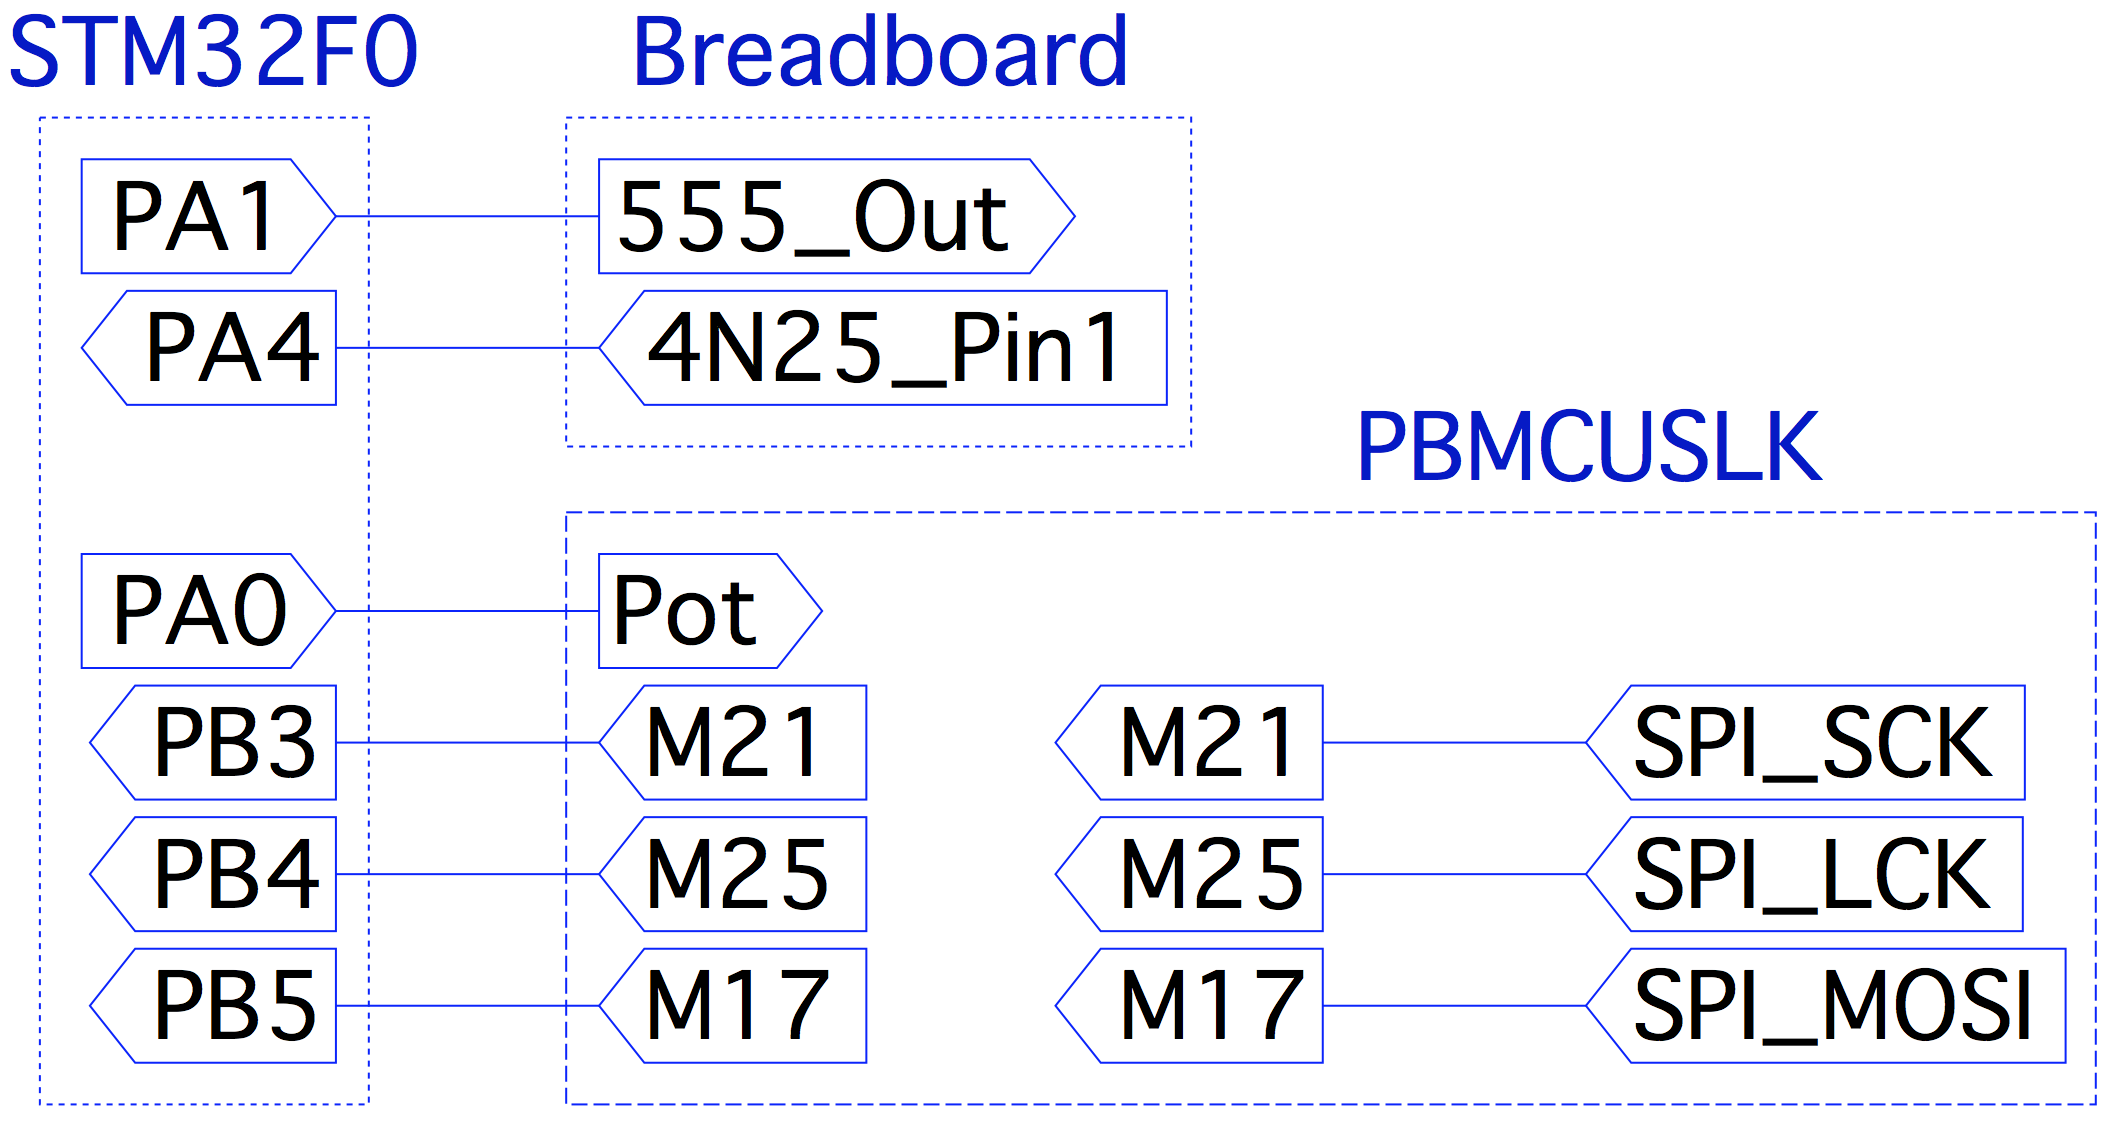
\includegraphics[width=0.7\linewidth]{../graphics/schematic_uc-to-project-board}
  \caption{External device connection summary}
  \label{fig:schematic_uc-to-project-board}
\end{figure}

\subsection{LCD}\label{sec:lcd}
The project board has an eight character by two row LCD for text display.
The LCD has a standard HD44780 control circuit that provides fourteen inputs.
Only six of the inputs - data lines 4 to 7, the RS pin and EN pin - are controllable by the user.
The hard-wired values for the driver are shown in Figure~\ref{fig:schematic_lcd}.

A down/up transition of the EN pin causes the LCD to accept and execute the current command or data on its data line.
The RS pin sets the interpretation of the value on the data pins.
If RS is low the data is a \textit{command} which can change the operating state of the LCD.
RS high indicates a \textit{data} word, such as a character to display.
This value is saved in the LCD's internal DDRAM~\cite{H:HD44780}.

\begin{figure}[tbph]
  \centering
  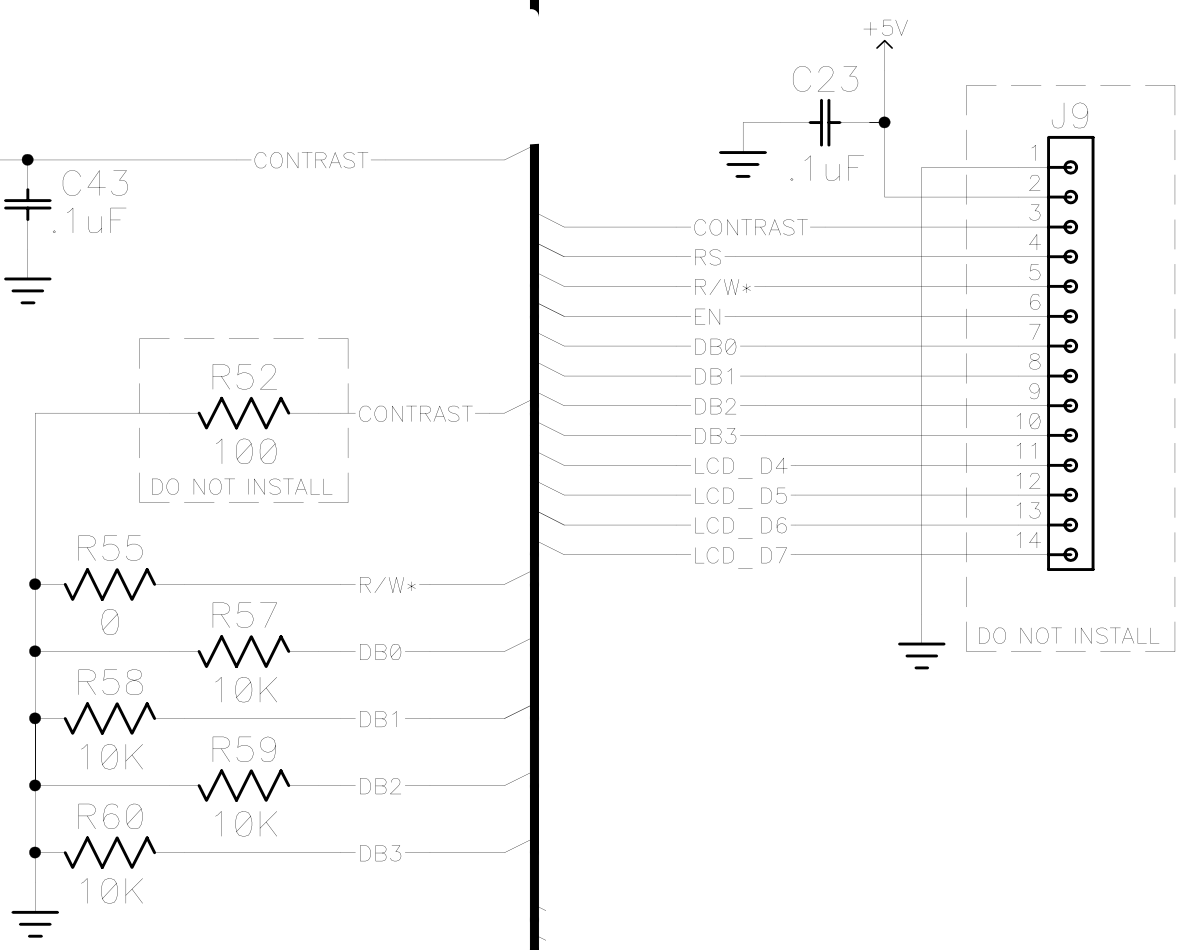
\includegraphics[width=0.7\linewidth]{../graphics/schematic_lcd}
  \caption{The HD44780 LCD driver only exposes the upper four data lines, RS and EN pins to the user~\cite[p. 3]{schematic:PBMCUSLK}}
  \label{fig:schematic_lcd}
\end{figure}

The user-controllable pins from the HD44780 are connected to an HC595 8-bit shift register.
This is a common practice because data can be loaded in to the shift register sequentially and then exposed to each line of the controller in parallel.
This reduces the number of connections from the board to the LCD driver at the cost of a slower transfer rate.
The connections between the project board, shift register and LCD driver are shown in Figure~\ref{fig:schematic_shift-reg}.

The MOSI line transfers signals from the microcontroller to the shift register input, A.
A down/up transition on the SCK line will move the data in registers QA through QG down one position and move the value on line A into QA.
If the LCK line is low the Qx outputs will hold their output values while their internal registers take on new values.
When LCK is set high the Qx outputs update to match their internal register values~\cite{TI:HC595}.

\begin{figure}[tbph]
  \centering
  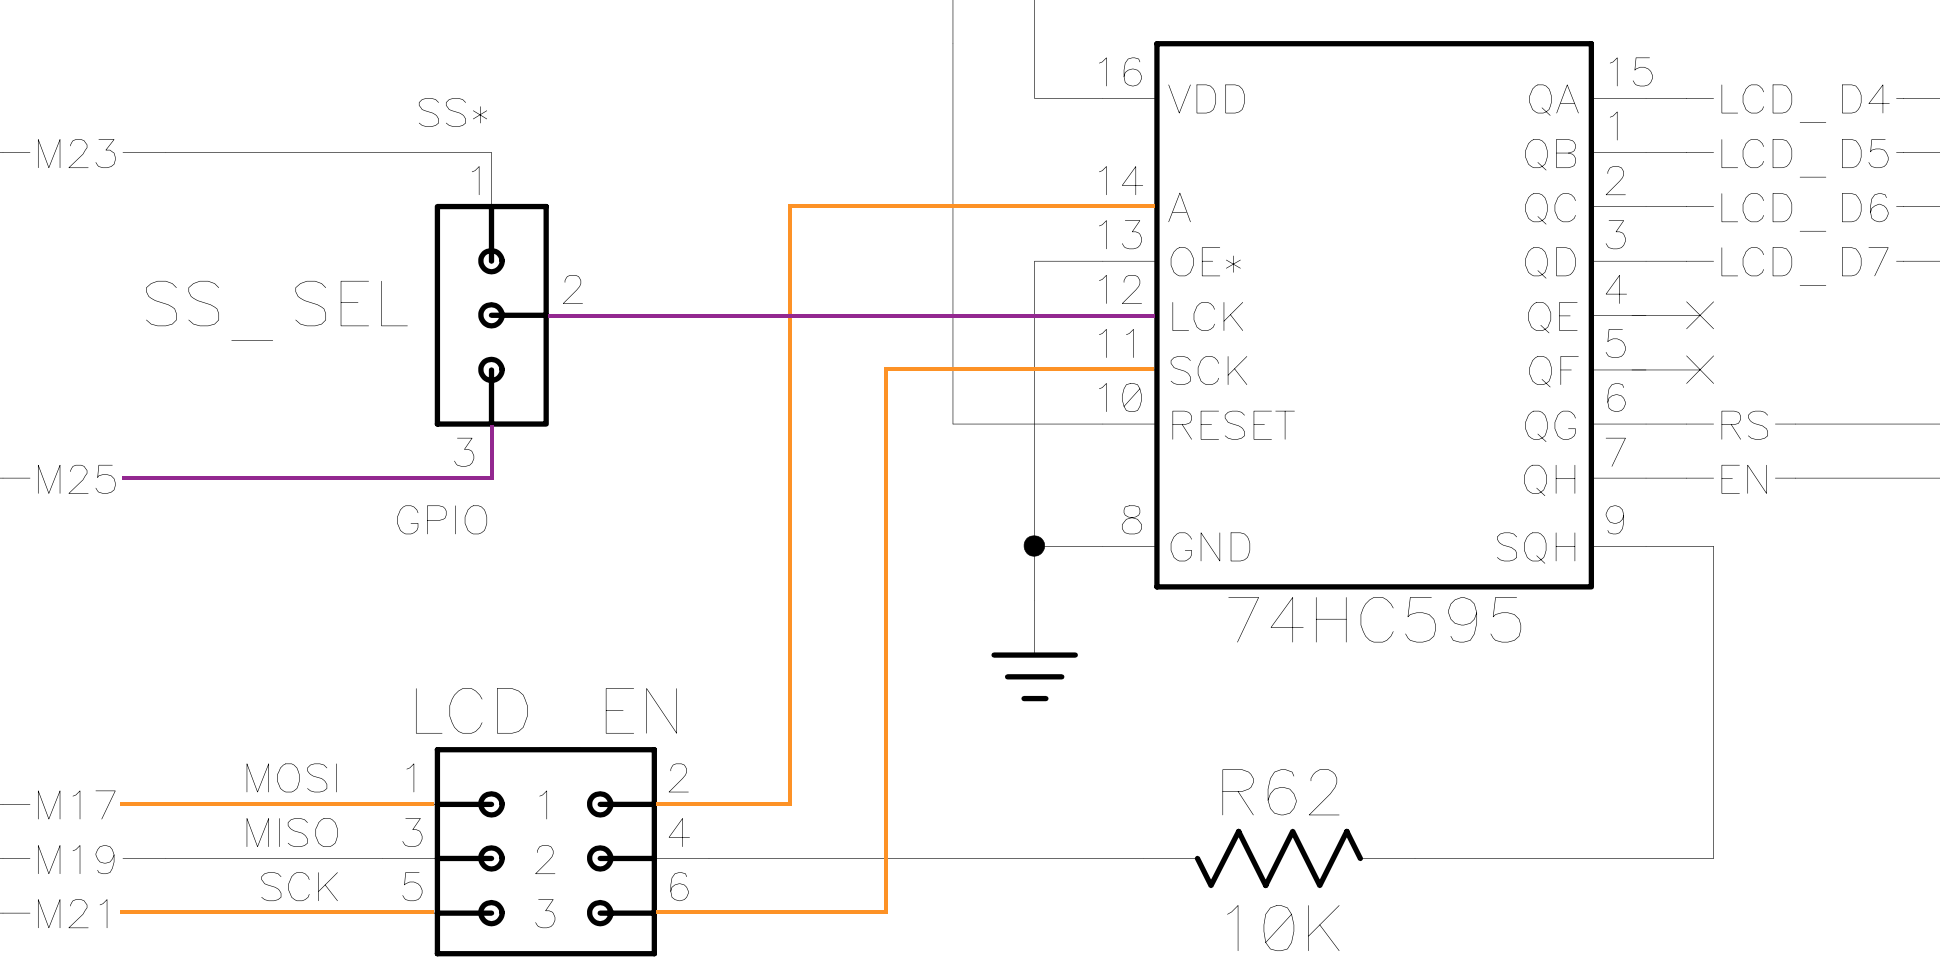
\includegraphics[width=0.7\linewidth]{../graphics/schematic_shift-reg}
  \caption{Detail of the SPI communication lines (orange) and shift register control line (purple)~\cite[p. 3]{schematic:PBMCUSLK}}
  \label{fig:schematic_shift-reg}
\end{figure}

All of the LCD control functionality is included in \texttt{lcd.c}, a reusable library of LCD interface functions.
Software configuration for SPI communication begins in \texttt{myGPIOB\_Init()} with setting GPIO pins PB3 and PB5 to operate in alternate function mode.
The F0 reference manual indicates that PB5 will be used for MOSI communication and PB3 for SCK control~\cite{STM:f0ref}.
PB4 is configured as a regular digital out and will be used to control LCK, the shift register output update pin.

\texttt{stm32f0xx\_spi.h} provides library functions for using the built-in SPI capabilities of the microcontroller.
The \texttt{SPI\_InitStruct} has a few notable values: SPI will be unidirectional with the microcontroller acting as master; data size is 8 bits, to match the size of the shift register, and; the baud rate prescaler is 256, the slowest possible transfer rate.
Normally, the R/$\overline{\text{W}}$ bit of the HD44780 can be set to read.
This exposes a flag that indicates if the LCD is ready to receive more data.
However, the project board grounds this pin, preventing the LCD from entering read mode (see Figure~\ref{fig:schematic_lcd}).
The ready status of the LCD is unknowable.
Since the microcontroller has a much faster clock speed than the HD44780 we assume the bottleneck will be on the receiver's end.

The microcontroller must follow a precise sequence of events to correctly expose data to the shift register and then the LCD controller.
Before sending data to the shift register the LCK pin is set low to ensure only valid words are exposed to the LCD controller.
Next, the SPI is checked to see if it can accept more data in its transmission queue.
When the queue is clear the library function \texttt{SPI\_SendData8(SPIx, word)} will send an 8-bit word into the shift register by controlling the MOSI and SCK values.
SPI flags are checked again to wait for transmission to finish.
When finished, LCK is set high and the new 8-bit word is exposed to the LCD controller.

The communication between the shift register and the LCD controller is less straight-forward because the LCD controller has two operating modes: 8-bit mode and 4-bit mode.
In 8-bit mode the controller reads values from \textit{all} data lines, including the grounded lines 0 to 3.
In 4-bit mode the controller ignores lines 0 to 3 and reads lines 4 to 7 as successive half-words, starting with the upper half.
Once the lower half is received the corresponding command is executed.

To send an 8-bit word to an LCD in 4-bit mode the word must be broken into upper and lower half-words.
As shown in Figure~\ref{fig:schematic_shift-reg}, the data lines correspond to the lower half of the shift register and the RS and EN lines correspond to the upper half.
Data is sent to the shift register in the following order:
\begin{enumerate}[nolistsep]
  \item Disable LCD, send high data
  \item Enable LCD, send high data
  \item Disable LCD, send high data
  \item Disable LCD, send low data
  \item Enable LCD, send low data
  \item Disable LCD, send low data
\end{enumerate}
Steps 1-3 load the upper half-word into the LCD and steps 4-6 send the lower half.
Toggling the LCD from Disable $\rightarrow$ Enable is what causes the word to be loaded.
Additionally, the RS bit is constant for all steps and indicates whether the data corresponds to a command or data word.

When the LCD boots from power off it loads its default configuration which, unfortunately, sets it in 8-bit mode~\cite{H:HD44780}.
By sending the word \texttt{0x2} to the LCD we set it to 4-bit mode and can continue with further configuration. (It's not always the case that the LCD is configured from a default state.
Consider debugging, where the LCD might already be in 4-bit mode when it tries to execute the initial configuration.
Section~\ref{sec:discussion} outlines a procedure for configuring the LCD from an unknown initial state.) Subsequent configuration commands enable two line display, hide the cursor and set the LCD to increment to the next character after one has been written.
Finally, the clear screen command is issued.

Some LCD commands, such as clear screen, require over \SI{1.5}{\milli\second} to complete.
This is longer than the minimum SPI baud rate.
Sending a command immediately after a slow command like clear screen will result in undefined behavior from the LCD.
As such, a \SI{2}{\milli\second} delays is inserted after the clear command.
Timer 3 is configured as a non-blocking timer.
When a delay is called the timer is polled until its internal counter expires.
This allows other time critical functions, such as input wave edge measurements, to interrupt the delay.

To display characters on the LCD the output character must be mapped to the corresponding entry on the LCD character table~\cite[p. 17]{H:HD44780}.
Thankfully, 8-bit representation of \texttt{char *} values for A-Z,a-Z map directly to the LCD table so explicit casting will give the correct value.
Digits 0-9 must be mapped to values starting at \texttt{0x30}, where \texttt{0x30} $\rightarrow$ 0, \texttt{0x31} $\rightarrow$ 1, and so on.

The last consideration for designing the LCD interface is its update interval.
Attempting to update the LCD too quickly, such as in the main program loop, quickly overflows the LCD's internal buffers and leads to undefined behavior.
A third timer, \texttt{TIM16} is configured to interrupt every \SI{250}{\milli\second}.
The interrupt handler writes new values for resistance and frequency to the LCD.
Since writing to the LCD involves sending data to the shift register six times for each \textit{character}, each with two polling loops, it is the slowest operation on the microcontroller.
It's also the least reliant on real-time execution since it's not trying to measure a continuously changing signal. \SI{250}{\milli\second} is infrequent enough to not hog the majority of CPU cycles but quick enough to seem responsive to a human user.

\subsection{ADC}\label{sec:adc}
The project board has a \SI{5}{\kilo\ohm} potentiometer (Figure~\ref{fig:schematic_pot}) that is connected to an analog input on the microcontroller.
As is common with potentiometers, the lower resistance value is significantly above \SI{0}{\ohm}.
With minimum resistance, the measured voltage on the potentiometer center lead is $\approx \SI{1.1}{\volt}$, indicating a minimum resistance of $\approx \SI{1.67}{\kilo\ohm}$.

\begin{figure}[tbph]
  \centering
  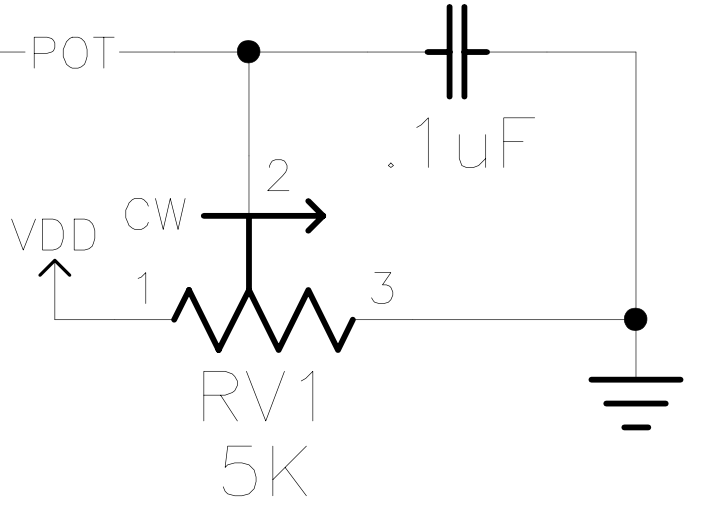
\includegraphics[width=0.4\linewidth]{../graphics/schematic_pot}
  \caption{Schematic of the project board potentiometer, $V_{DD} = \SI{3.3}{\volt}$~\cite{FS:PBMCUSLK}.}
  \label{fig:schematic_pot}
\end{figure}

PA0 is one of sixteen available analog inputs with ADC converters on the microcontroller~\cite[ch. 13]{STM:f0ref}.
During initialization, \texttt{myGPIOA\_Init()} configures PA0 as an analog input. \texttt{myADC\_Init()} executes the ADC specific initialization procedure outlined in the f0 reference manual~\cite[ch. 13]{STM:f0ref}.
After the reference clock is enabled for the ADC, the \texttt{ADC\_CR\_ADCAL} flag is set in the ADC control register.
This flag begins the built-in ADC calibration procedure which maps the input voltage range, \SIrange{1.1}{3.3}{\volt}, to the default 12-bit resolution, values 0 to 4095.
Hence, when the ADC voltage is converted to a resistance it represents a \textit{notional} resistance value rather than the \textit{actually existing} resistance value of the potentiometer.

When the calibration completes the ADC is set to operate in continuous conversion and overrun modes.
Continuous conversion will automatically start a new conversion once the ADC value is dereferenced.
Overrun mode sets the ADC to overwrite its buffer when full.
If this isn't set, a full ADC buffer will cause an overrun error and crash both the ADC \textit{and} DMA controllers without proper handling.

Finally, the enable flag is send to the ADC control register.
If the configuration is valid the \texttt{ADC\_ISR\_ADRDY} flag is set, indicating that the ADC is ready to accept conversion requests.

Conversion requests are issued from the main loop of the program.
Each loop cycle, the conversion request is sent with \texttt{ADC\_CR\_ADSTART}.
The program polls until the end of conversion flag, \texttt{ADC\_ISR\_EOC}, is set.
When the conversion is complete, the program resets the end of conversion flag and reads the 12-bit converted value from the ADC data register \texttt{ADC1->DR}.
This sequence is encapsulated in \texttt{getPotADCValue()}.

\subsection{555 Timer circuit}\label{sec:circuit}
The analog output voltage generated by the microcontroller is from a pulse wave modulated (PWM) signal.
This signal contains an AC component that would result in unstable operation operation of the 555 timer.
To eliminate the AC component, the PWM signal is connected to an optocoupler.
The input signal modulates the brightness of an internal LED.
The LED brightness controls the gain of an internal NPN BJT.
Since the brightness of the LED is not affected by the AC component the result is a DC signal on the BJT.
Figure~\ref{fig:schematic_opto-to-555} shows the connection of the optocoupler to a 555 timer in astable operation.

\begin{figure}[tbph]
  \centering
  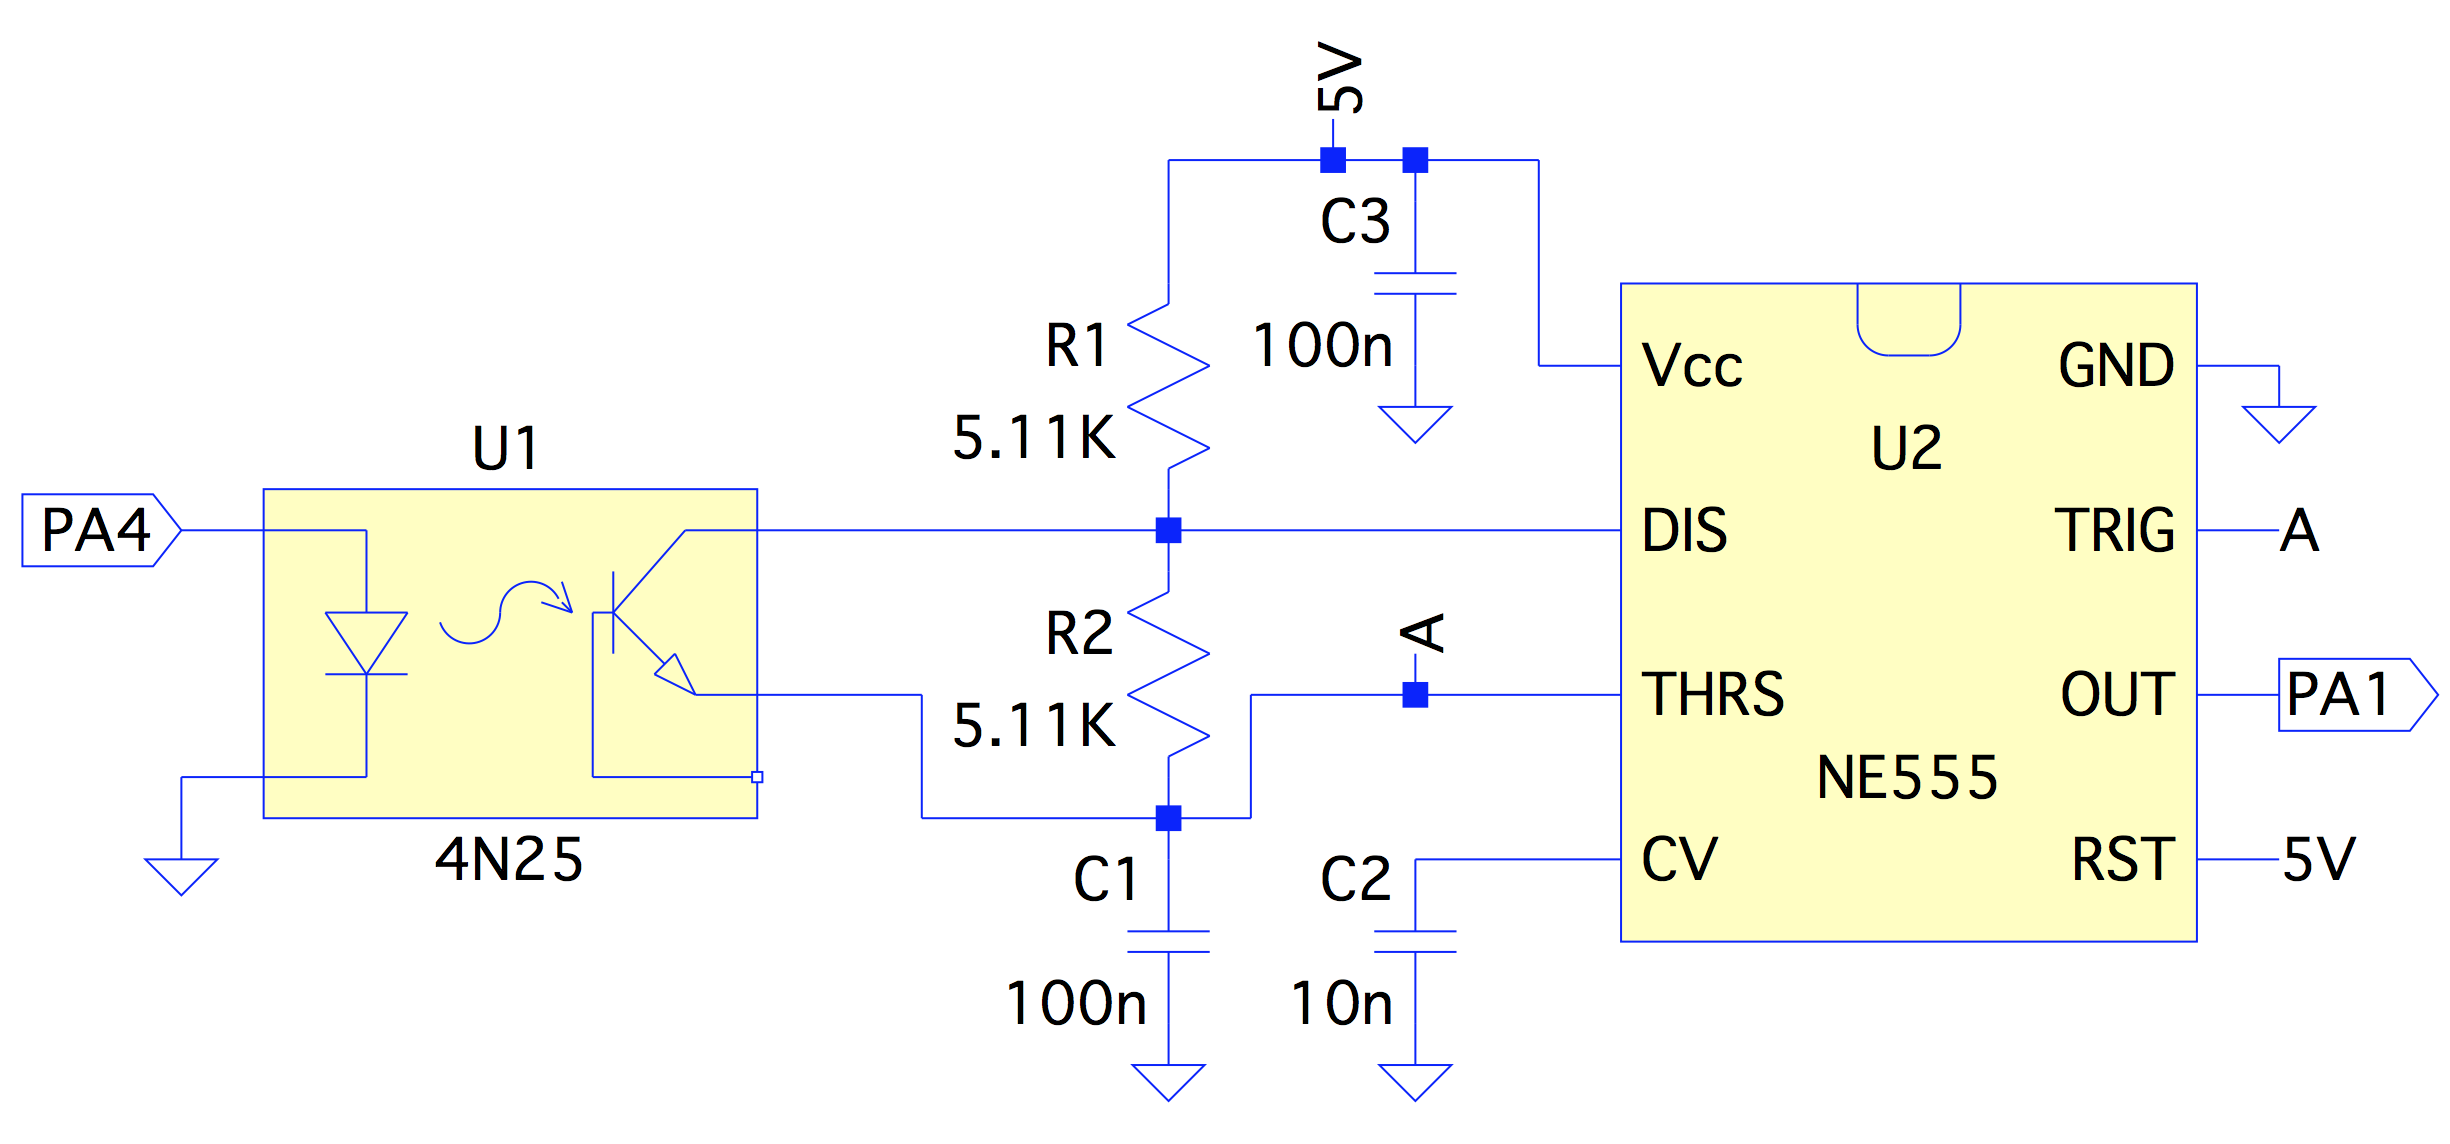
\includegraphics[width=0.8\linewidth]{../graphics/schematic_opto-to-555}
  \caption{An optocoupler allows a PWM signal to control the output frequency of a 555 timer in astable operation}
  \label{fig:schematic_opto-to-555}
\end{figure}

With this astable configuration, the output signal is a square wave with the frequency determined by~\cite{STM:555}:
\begin{equation}\label{eqn:555-freq}
  f = {1.44 \over \left(R_1 + 2R_2\right) C_1}.
\end{equation}
Changing the gain of the NPN BJT in the optocoupler changes the voltages on either side of $R_2$, thus altering $R_2$'s value in \eqref{eqn:555-freq}.

This circuit was constructed and tested in isolation using the potentiometer voltage as an input (instead of PA4) and an oscilloscope as an output (instead of PA1).
Testing confirmed the relationship expected in \eqref{eqn:555-freq}, that $f \propto R_2^{-1}$.
See Section~\ref{sec:test-timer} for more information on the testing procedure.

Testing the timer operation in isolation also reveal a range of input voltages that did not affect the timer output.
For input voltages \SIrange{0}{1.07}{\volt} there was no change in timer frequency.
This is because the optocoupler has two internal diodes: one in the LED and another in the BJT.
This is consistent with the forward voltage listed in the 4N35 datasheet: \SIrange{0.9}{1.7}{\volt} with a typical value of \SI{1.3}{\volt}~\cite{V:4N35}.
As a result of this deadband voltage range the DAC will only output values above \SI{1.07}{\volt} so that all values of the potentiometer generate a unique timer voltage.

\subsection{DAC}\label{sec:dac}
Compared to the LCD controller and ADC, the DAC is simple to initialize and use.
PA4 is the default connection for DAC output so it's configured as an analog output in \texttt{myGPIOA\_Init()}.
The DAC is initialized by enabling its associated clock and setting the enable bit in its control register.
The main loop sets the DAC output voltage by writing a 12-bit value to \texttt{DAC->DHR12R1}, the DAC data register which is 12-bit and right aligned.
Conveniently, this is the same alignment as the ADC value.

The function \texttt{applyOptoOffsetToDAC()} shifts the 12-bit value read from the ADC to output voltages \SIrange{1.07}{3.3}{\volt}, which is the range of voltages that change the 555 timer frequency.
